\documentclass[11pt,a4paper]{article}

\usepackage[margin=1.5cm]{geometry}
\usepackage{amsmath, amssymb, graphicx, setspace, caption, subcaption}
\usepackage{helvet}
\renewcommand{\familydefault}{\sfdefault} % Arial-like font
\usepackage{booktabs}
\usepackage{hyperref}
\usepackage{amsfonts}
\usepackage{graphicx}
\setstretch{1.1}

\begin{document}

    \begin{center}
    {\Large \textbf{Momentum Long-Short Stock Picking Strategy}}
    \end{center}
    \vspace{-0.5em}

    \section*{1. Strategy Overview}

    \paragraph{}
    Our equity strategy delivers alpha through daily prediction and positioning across 50 of the largest US stocks, to capture relative performance while minimizing market risk. The strategy leverages a multi-dimensional dataset combining fundamental analyst forecasts, systematic risk factors, technical price patterns, and real-time market regime indicators including volatility indices and sector rotation signals.
    Each trading day, our machine learning framework employs two separate models: one predicts direction and another estimates magnitude, which are then combined for better accuracy. Our models analyzes over 100 engineered features to identify the most attractive long and short opportunities. Our scoring and allocation methodology transform these predictions into optimal position weights, which ensure risk-adjusted portfolio construction. This daily rebalancing approach captures short-term inefficiencies and momentum patterns, while our diversified feature set ensures strong performance across varying market cycles.

    \begin{figure}[h!]
        \centering
        \begin{minipage}[t]{0.70\textwidth}
        \begin{minipage}[t]{0.70\textwidth}
            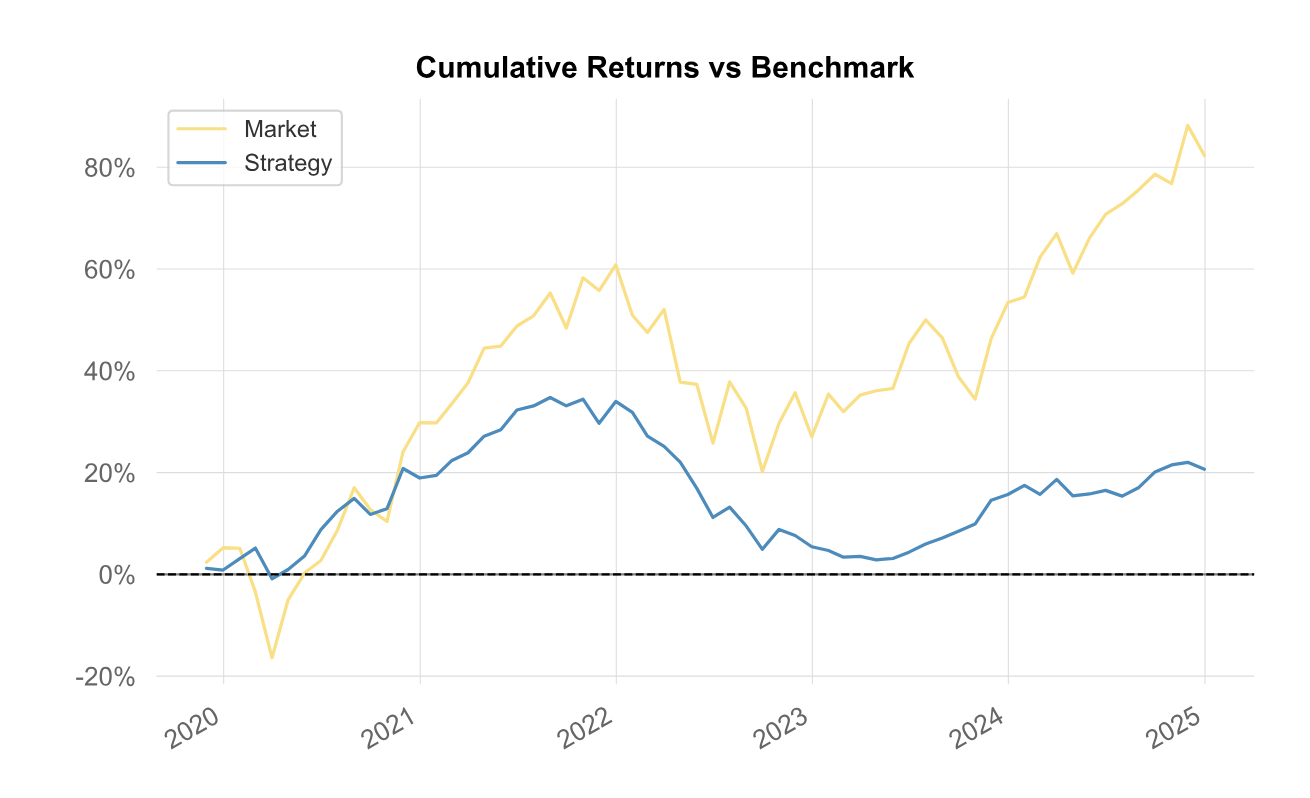
\includegraphics[width=\linewidth]{Strategy.png}
            \vspace{-0.5em} % fine-tune vertical spacing under image
            \label{fig:returns_vs_benchmark}
        \end{minipage}
        \hfill
        \begin{minipage}[t]{0.28\textwidth}
            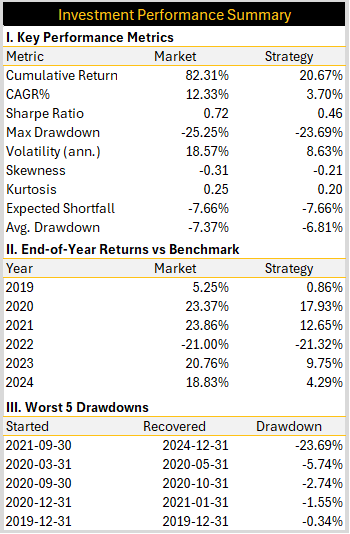
\includegraphics[width=\linewidth]{Key Metrics.png}
            \vspace{-0.5em}
            \label{fig:key_metrics}
        \end{minipage}
        \vspace{-1.2em} % reduces extra white space below the figure block
    \end{figure}

    \paragraph{Performance Summary.}
    While the strategy does not outperform the market in cumulative returns, it offers lower annualized volatility and smaller drawdowns. This is attractive for investors that prioritize stability and capital preservation who would trade off higher potential returns for lower risk exposure.
    \vspace{1em}
    \section*{2. Machine Learning Strategy}

    \paragraph{Notation.}
    For stock $i$ on date $t$, let $\mathbf{x}_{i,t}\in\mathbb{R}^{K}$ be the standardized feature vector ($K\approx 100$), and let
    $y_{i,t+1}$ denote the next-day log return. The sample is split chronologically into in-sample (IS, 65\%) and out-of-sample (OOS, 35\%), and 10-fold rolling windows are used inside IS for hyperparameter calibration while preserving temporal order.

    \subsection*{2.1 Models and Training}

    \textbf{Directional model (classification).}
    Following the course manual, logistic regression models the probability that the next-day return is positive as
    \[
        p_{i,t} = P(y_{i,t+1} = 1 \mid \mathbf{x}_{i,t})
        = \frac{\exp(\beta^{\text{log}}_0 + \boldsymbol{\beta}^{\text{log}\top}\mathbf{x}_{i,t})}
        {1 + \exp(\beta^{\text{log}}_0 + \boldsymbol{\beta}^{\text{log}\top}\mathbf{x}_{i,t})},
    \]
    equivalently,
    \[
        \log\!\left(\frac{p_{i,t}}{1 - p_{i,t}}\right)
        = \beta^{\text{log}}_0 + \boldsymbol{\beta}^{\text{log}\top}\mathbf{x}_{i,t}.
    \]
    Parameters are estimated by maximum likelihood with an elastic-net penalty. The SAGA solver with early stopping is used, and the optimal regularization hyperparameters are selected by minimizing the average classification error across rolling validation folds.

    \medskip
    \textbf{Magnitude model (regression).}
    For return magnitude forecasting, a linear regression estimates the conditional mean of next-day returns:
    \[
        y_{i,t+1}
        = \beta^{\text{lin}}_0 + \boldsymbol{\beta}^{\text{lin}\top}\mathbf{x}_{i,t} + \varepsilon_{i,t},
        \qquad
        \hat{y}_{i,t+1} = \hat{\beta}^{\text{lin}}_0 + \hat{\boldsymbol{\beta}}^{\text{lin}\top}\mathbf{x}_{i,t}.
    \]
    Coefficients are obtained by minimizing the penalized residual sum of squares under an elastic-net penalty. Tuning parameters are chosen via rolling cross-validation by minimizing RMSE.

    \medskip
    \textbf{Rolling cross-validation (temporal integrity).}
    For fold $f=1,\dots,F$,
    \[
        \text{train}_f=[t_f,\, t_f+T_{\text{train}}),
        \quad
        \text{val}_f=[t_f+T_{\text{train}},\, t_f+T_{\text{train}}+T_{\text{val}}),
    \]
    with $T_{\text{train}}\approx 0.6$ and $T_{\text{val}}\approx 0.2$ of the IS window. Each fold advances by a fixed step, ensuring validation always follows training and no look-ahead bias is introduced.

    \subsection*{2.2 Signal Construction and Ensemble}

    \textbf{Binary model signals.}
    Directional (probability) and magnitude (expected return) thresholds define preliminary long/short flags:
    \[
        \begin{aligned}
            \text{Long}^{(\mathrm{log})}_{i,t} &= \mathbb{1}[\,p_{i,t} > 0.55\,],
            &\quad \text{Short}^{(\mathrm{log})}_{i,t} &= \mathbb{1}[\,p_{i,t} < 0.45\,],\\
            \text{Long}^{(\mathrm{lin})}_{i,t} &= \mathbb{1}[\,\mu_{i,t} > 0.001\,],
            &\quad \text{Short}^{(\mathrm{lin})}_{i,t} &= \mathbb{1}[\,\mu_{i,t} < -0.001\,].
        \end{aligned}
    \]

    \textbf{Ensemble agreement (confirmation filter).}
    A trade is eligible only if both models agree on direction:
    \[
        \text{Long}_{i,t}=\text{Long}^{(\mathrm{log})}_{i,t}\land \text{Long}^{(\mathrm{lin})}_{i,t},\qquad
        \text{Short}_{i,t}=\text{Short}^{(\mathrm{log})}_{i,t}\land \text{Short}^{(\mathrm{lin})}_{i,t}.
    \]
    This confirmation step reduces false positives and concentrates exposure on high-confidence predictions.

    \medskip
    \textbf{Composite scores (ranking).}
    We convert $(p_{i,t},\mu_{i,t})$ into a scalar score $s_{i,t}$ for ranking and sizing:
    \[
        \boxed{
            \begin{aligned}
                \mathrm{S1:}\;\; s_{i,t} &= p_{i,t}\,\mu_{i,t},\\
                \mathrm{S2:}\;\; s_{i,t} &= (p_{i,t}-0.5)\,\mu_{i,t},\\
                \mathrm{S6:}\;\; s_{i,t} &= (2p_{i,t}-1)\,|\mu_{i,t}|.
            \end{aligned}}
    \]
    S1 captures the joint expected value, S2 emphasizes the confidence margin, and S6 separates direction (through $2p-1$) from conviction ($|\mu|$).
    If the models disagree, $s_{i,t}=0$ and the observation is excluded from trading.

    \subsection*{2.3 From Scores to Portfolio Weights}

    Let $\mathcal{L}_t=\{i:\text{Long}_{i,t}=1\}$ and $\mathcal{S}_t=\{i:\text{Short}_{i,t}=1\}$.

    \begin{itemize}
        \setlength\itemsep{2pt}
        \item \textbf{A1 Equal-weighted:}
        $w_{i,t}= \frac{1}{|\mathcal{L}_t|}$ for $i\in\mathcal{L}_t$;
        $w_{i,t}= -\frac{1}{|\mathcal{S}_t|}$ for $i\in\mathcal{S}_t$.
        \item \textbf{A2 Rank-weighted:}
        Within each side, $w_{i,t}\propto \mathrm{rank}(s_{i,t})$ (higher score $\Rightarrow$ larger weight).
        \item \textbf{A3 Quantile:}
        Trade only extreme scores:
        $w_{i,t}\propto \mathbb{1}[\,s_{i,t}\ge \tau^{\text{long}}_{0.8}\,]$ (long)
        and
        $w_{i,t}\propto -\mathbb{1}[\,s_{i,t}\le \tau^{\text{short}}_{0.2}\,]$ (short).
        \item \textbf{A4 Score-weighted:}
        $w_{i,t}\propto s_{i,t}$ (direction from sign, size from magnitude).
        \item \textbf{A5 Inverse-volatility:}
        Compute $\sigma_{i,t}$ (20-day rolling volatility); set pre-weights $\tilde w_{i,t}\propto \frac{\mathrm{sign}(s_{i,t})}{\sigma_{i,t}}$ for eligible names.
    \end{itemize}

    \textbf{Normalization and constraints.}
    Weights are scaled to maintain dollar neutrality and capped at 5\% per position:
    \[
        \sum_{i\in\mathcal{L}_t} w_{i,t}=1,\qquad \sum_{i\in\mathcal{S}_t} |w_{i,t}|=1,\qquad |w_{i,t}|\le 0.05,
    \]
    so that gross exposure is 2.0 and net exposure is 0.

    \subsection*{2.4 Evaluation and Selection}

    \textbf{In-sample model and strategy selection.}
    We backtest all $3\times 5=15$ (score, allocation) combinations on IS data and select
    \[
        (\mathrm{score}^\star,\mathrm{alloc}^\star)=\arg\max \;\mathrm{Sharpe}_{\mathrm{IS}}.
    \]
    Rolling cross-validation ensures parameter tuning is performed only with past data, while degradation from IS to OOS is reported to evaluate robustness.

    \medskip
    \textbf{Out-of-sample performance.}
    With models fixed at IS-optimal hyperparameters and $(\mathrm{score}^\star,\mathrm{alloc}^\star)$ locked in, daily portfolio returns are
    \[
        r_{p,t+1}=\sum_{i} w_{i,t}\, r_{i,t+1}, \qquad
        \mathrm{Sharpe}=\frac{\mathbb{E}[\,r_{p}-r_f\,]}{\mathrm{sd}(r_{p})}\sqrt{252}.
    \]

    \vspace{}
    \section*{3. Discussion: Strengths and Limitations}

    \paragraph{}Using linear model frameworks provides clear feature-prediction mappings and interpretability, although they cannot capture non-linear feature interactions. Sliding window cross-validation maintains temporal integrity, and applying elastic net regularization balances feature selection and limits overfitting. However, the static architecture means models are not retrained in forward-looking scenarios, causing performance drift over time.

    \paragraph{}
    The dual-model architecture creates reliability by filtering uncertain predictions. Training models across all stocks limits overfitting, though this sacrifices potential accuracy gains from stock-specific calibration. Daily rebalancing enables the capture of short-term market inefficiencies, but the strategy does not assume transaction costs, bid-ask spreads, or market impact. Also, perfect liquidity assumptions may be unrealistic for large positions.

    \paragraph{}
    The research-based parameter selection process relies on systematic hyperparameter tuning and academic literature (Hastie et al. (2009)) rather than arbitrary fixed values, however, the approach may overfit to established academic assumptions or historical relationships that no longer hold in current markets. Additionally, the strategy lacks a separate regime detection model that could dynamically select optimal feature sets and weights for different market regimes.

\end{document}
